We extended the current official Raft visualizer
to emulate the full protocol and we integrated the latest published variation
and fixes (Figure~\ref{fig:final}).

\subsection{Protocol}
Now the simulator support \emph{Cluster membership changes}.
    Addition and removal of a follower and removal of the leader
    from the cluster via the single-server mutation
    algorithm proposed by Ongaro in his Ph.D. thesis~\cite{ongaro2014consensus}.

The fix for single-server algorithm was also backported;
    as discussed at the \#raft-dev mailing list~\cite{bug} with this
    algorithm could happen double leadership and committed history rewrite.
    The fix we implemented is to write in the log a \texttt{NOOP} message
    every time a server becomes a \emph{leader}.

We also implemented the safety check for Disruptive servers:
    Follower servers ignore \texttt{voteRequest} if it has heard from the
    current limit within \texttt{MIN\_ELECTION\_TIMEOUT}; prescribed in the
    section 4.2.3 of the Ongaro's thesis.

\subsection{Simulation}
We added the concept of \texttt{network noise}; the system simulate the noise
on the network dropping each message with a probability set by the user.

A \emph{cluster configuration changes queue} was added to allow the user to submit
multiple configuration change requests. In the thesis it is not clear whether it is the
leader to have to buffer for the changes request or the client trying up to succeed.
We decided that it is duty of the leader; this means that when the leader changes
pending operations are lost.

\subsection{Internals}
To support the new protocol functionalities we had to modify the
\texttt{checkpoint} snapshot format and the main loop.
In order to allow transparently replay/rollback/playback we have also to
modify the rendering phase to take in account the possibility that
servers can join and leave, particularly challenging was to deterministically decide
when it is safe to remove a server from the graphic and thus from the simulation.
We decided to remove it when no one server has got it in the \texttt{peers} list.


\subsection{Interface}
For the timing issue discussed in Section~\ref{sec:internals} we limited the
simulation speed into a reasonable range.
The log table has been rewritten to support an infinite log and
now features also the auto scroll.
To avoid confusion the ``leader only'' fields in the state modal of the
follower servers have been hidden and a legend was added to explain the
otherwise cryptic symbols in the log table. Moreover, now, each log entry
is represented differently on the basis of its nature (\texttt{NOOP}, Config
change message, user value).
We obviously added controls for the feature we introduced in the Protocoll,
we thus added a slider to set the \emph{network noise}, a \emph{server add}
button and a voice to the context menu for server removal and finally
a new table to visualize the cluster configuration changes queue.
Besides that few minor bug were fixes.

\begin{figure}[h]
    \centering
    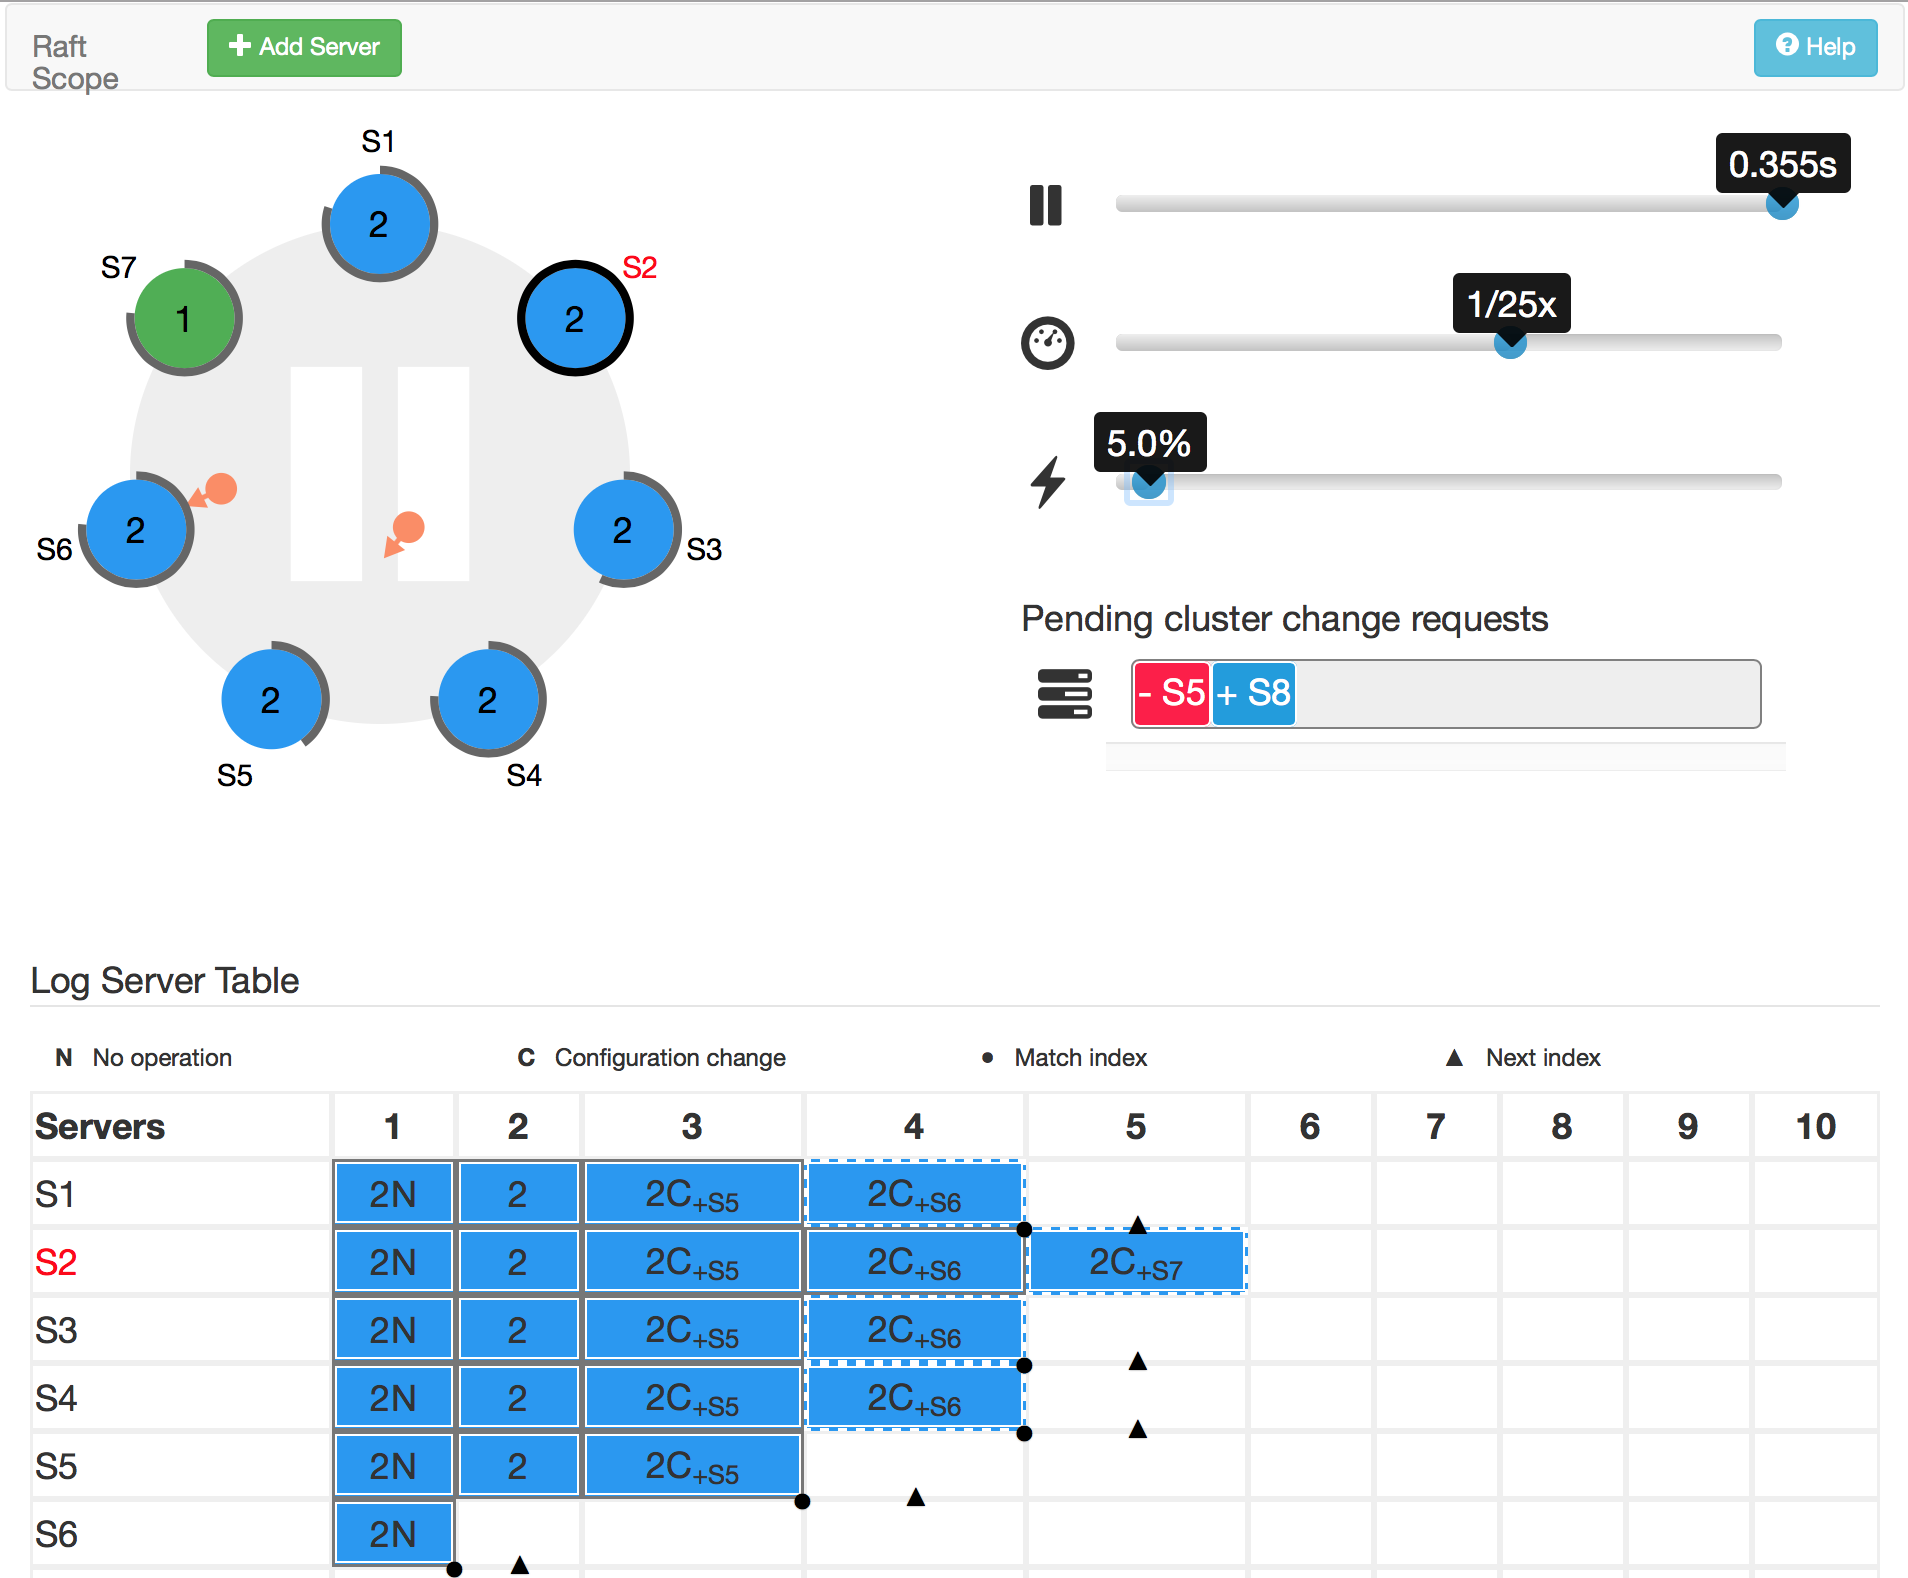
\includegraphics[width=0.9\linewidth]{our.png}
    \caption{Original}\label{fig:final}
\end{figure}

\subsection{Non implemented functionalities}
The \emph{leadership transfer extension} described in Section~3.10 of the thesis
was not implemented since it was never implemented or evaluated by the authors.

We did not implemented \emph{Joint consensus} since the one implemented is as
powerful as it is, but it is also simpler, more understandable and it is
the one the author indicated as preferred.
